\documentclass[]{article}

\usepackage{lmodern}
\usepackage[T1]{fontenc}
\input{H_structue}
\usepackage[a4paper, margin=1.2in]{geometry}
\definecolor{cover}{RGB}{230, 194, 24}
\newcommand{\dquad}{\quad\quad}
\newcommand{\tquad}{\quad\quad\quad}
\newcommand{\fquad}{\quad\quad\quad\quad}
\begin{document}


%----------------------------------------------------------------------------------------
%	TITLE PAGE
%----------------------------------------------------------------------------------------
\begingroup
\AddToShipoutPicture*{\put(0,0){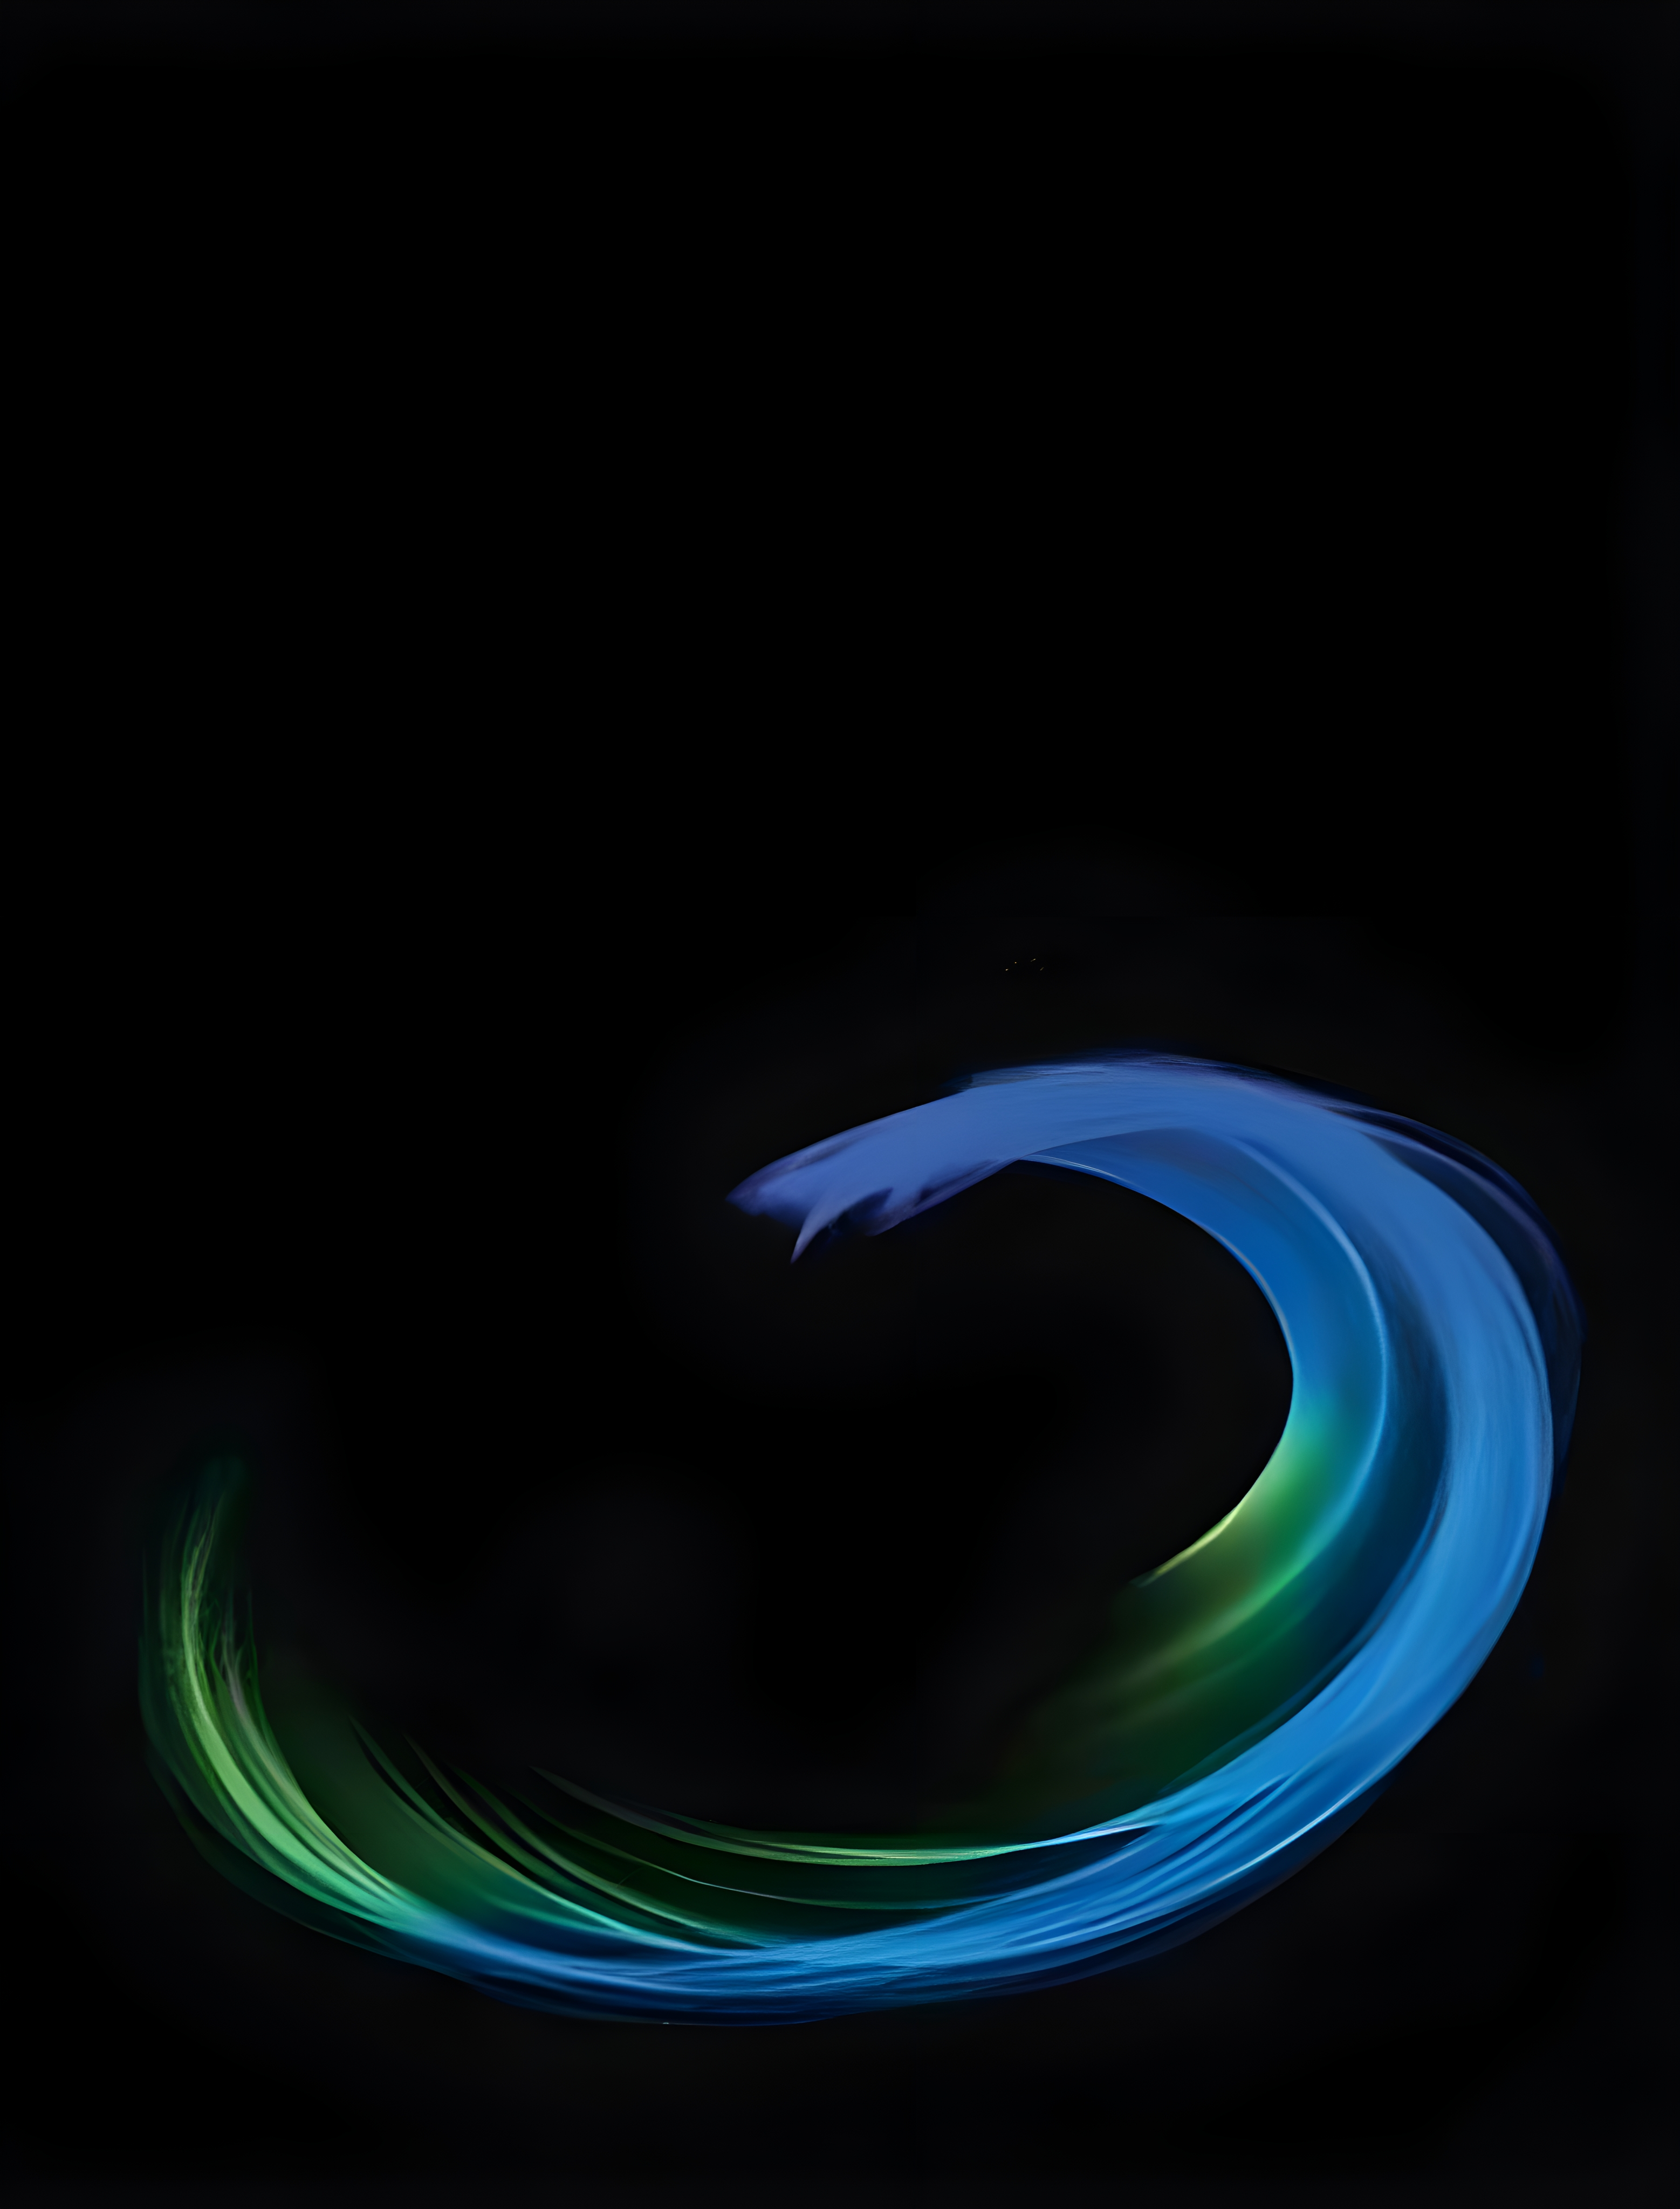
\includegraphics[width=\paperwidth,height=\paperheight]{Cover1.jpg}}}
\par\sffamily\selectfont
\color{cover}
\fontsize{80pt}{0}\selectfont Partial\par
\fontsize{80pt}{0}\selectfont Differential\par
\fontsize{80pt}{0}\selectfont Equations\par
\begin{center}
    {\LARGE 01356 Spring 2023}\par
    \vspace*{1cm}
    {\Huge Lecture Notes}\par       
\end{center}
\color{white}
\vspace*{4.5cm}
\fontsize{22pt}{0}\selectfont Lecturer: Prof. Mahmoud M. El-Borai\par
\fontsize{22pt}{0}\selectfont Prepared by: Ossama Abdelwahed And\par
\hspace*{4cm}
\fontsize{22pt}{0}\selectfont Ahmed.M.Habib\par
\endgroup

\newpage

\tableofcontents

\newpage

\section{Introduction}
The main goal of many scientfic displines can be summerized to the following:

\begin{enumerate}
\item Formulate a set of mathematical equations to model a phenomena of intrest
\item Analyze solutions to these equations in order to extract information and make predictions.
\end{enumerate}

The result of 1 is often a system of partial differential equations, thus the second becomes solving those partial differential equations.
\par
A partial differential equation (PDE) is is a differential equation containing partial derivatives of the dependent variable with repect to more than one independent variable.

\subsection{Order of PDE}
The order of a PDE is determined by the highest derivative in the equation.
\begin{align*}
\frac{\partial u}{\partial t} + {(\frac{\partial u}{\partial x})}^2 &= 0 \ \ \ \ \Longrightarrow  \text{First order}
\\
\frac{\partial^4 u}{\partial y^4} + \frac{\partial u}{\partial x} &= c \ \ \ \ \Longrightarrow  \text{Fourth order}
\end{align*}
do not mistake the order of the PDE with its degree, the degree of the PDE is the highest exponent appearing in the equation.
\subsection{Linearity} 
A linear PDE is one that is of first degree in all of its field variables and partial derivatives.
\begin{align*}
\frac{\partial u}{\partial t} + \frac{\partial u}{\partial x} &= 0 \dquad \text{linear}
\\
\frac{\partial^4 u}{\partial y^4} + \frac{\partial u}{\partial x} &= y \dquad \text{linear}
\\
\frac{\partial u}{\partial t} + {(\frac{\partial u}{\partial x})}^2 &= 0 \dquad \text{nonlinear}
\\
\frac{\partial^3 u}{\partial x^3} + {(\frac{\partial^2 u}{\partial y^2})}^5 &= \sin(x) \dquad \text{nonlinear}
\end{align*}

a linear operator can be defined for any linear equation, taking the first equation in the previous list, the linear operator $L$ can be defined as.
\[
L = \frac{\partial }{\partial t} + \frac{\partial u}{\partial x}
\]
and the equation can be written as.
\[
    L(u)=0    
\]

\subsection{Homogeneity}
Let $L$ be a linear operator. Then a linear partial differential equation can be written in the form.
\[
    L(u) = f(x_1,x_2, \dots , t)    
\]
if $f = 0$ then the equation is homogeneous, otherwise it is inhomogeneous.
\begin{align*}
\frac{\partial u}{\partial t} + \frac{\partial u}{\partial x} &= 0 \dquad \text{homogeneous}
\\
\frac{\partial^4 u}{\partial y^4} + \frac{\partial u}{\partial x} &= y \dquad \text{inhomogeneous}
\end{align*}

\newpage

\subsection{Boundry Conditions}
\ \ 
\begin{definition}{Boundary conditions}
    are constraints necessary for the solution of a boundary value problem.
\end{definition}
\begin{definition}
    boundary value problem is a differential equation to be solved in a domain on whose boundary the function is known.
\end{definition}
We will be intrested in one type of boundry conditions in this course which is the Drichlet Conditions, specifies the value that the unknown function needs to take on along the boundary of the domain. For example, the Laplace equation on a circle with drichlet condition will be.
\[
    \nabla^2 u(x) = 0 \quad \forall x \in G    
\]
\[
    u(x) = f(x) \quad \forall x \in G    
\]
\begin{center}
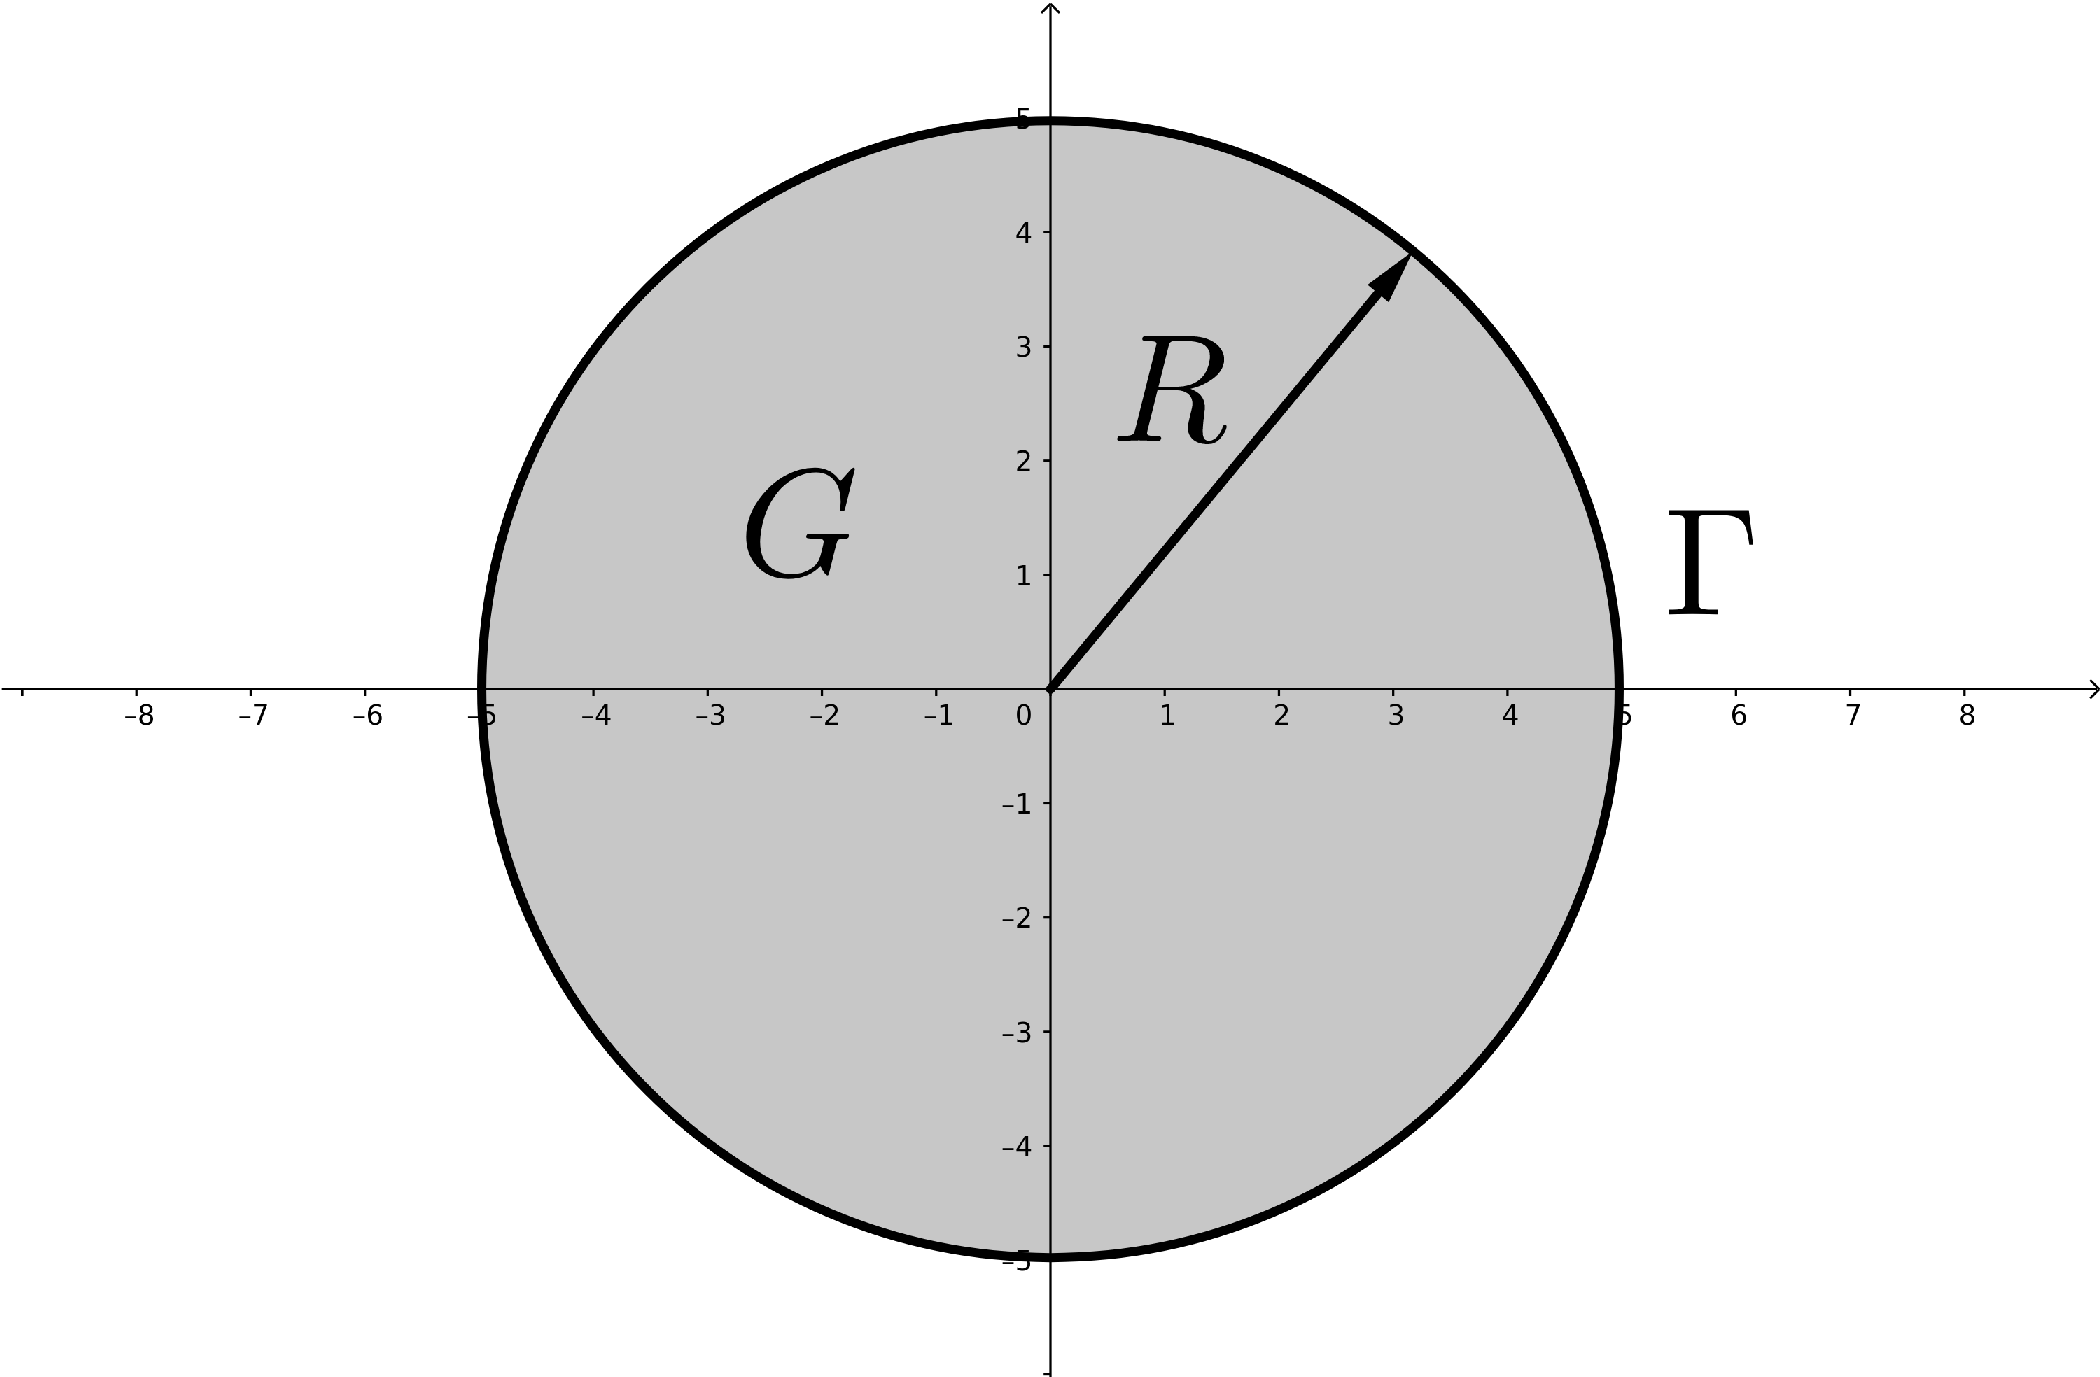
\includegraphics[scale=0.1]{laplacecircle.png} 
\end{center}
\[
    G = \left\lbrace (x,y):x^2+y^2 < R^2 \right\rbrace  \;\;\;\;\;\;\;\;\;\ \Gamma = \left\lbrace (x,y):x^2+y^2 = R^2 \right\rbrace    
\]
\begin{definition}
    Drichlet problems are problems that has only boundry conditions
\end{definition}
\subsection{Intial Condition}
\
\begin{definition}
    The initial condition is a condition that a solution must have at only on instant of time, which is the starting time as it can be found expremintally.
\end{definition}
An example is the heat equation with intial condition.
\[
    \frac{\partial u(x,t)}{\partial t}  = c^2 \frac{\partial u(x,t)}{\partial x}
\]
\[
    u(x,0) = f(x)
\]
\begin{definition}
    Cauchy problems are problems that has only intial conditions
\end{definition}
\subsection{Equations of Mathematical Physics}
The most frequently encountered equations in physics are the following
\begin{enumerate}
\item Heat Equation
\[
    \frac{\partial u(x,t)}{\partial t} = c^2 \frac{\partial^2 u(x,t)}{\partial x^2}    
\]
\item Wave Equation 
\[
    \frac{\partial^2 u(x,t)}{\partial t^2} = c^2 \frac{\partial^2 u(x,t)}{\partial x^2}    
\]
\item Laplace's Equation
\[
    \nabla^2 u(x) = \frac{\partial^2 u(x)}{\partial x^{2}_{1}} + \frac{\partial^2 u(x)}{\partial x^{2}_{2}} + \frac{\partial^2 u(x)}{\partial x^{2}_{3}} + \cdots = 0    
\]
\end{enumerate}

\newpage

\section{Canonical Form}
Consider the following PDE with variable coefficients. We are aiming to transform this equation into its canonical form
\begin{equation}
A\left(x,y\right)\frac{\partial^2 u\left(x,y\right)}{\partial x^2} + 2B\left(x,y\right)\frac{\partial^2 u\left(x,y\right)}{\partial x\partial y}+C\left(x,y\right)\frac{\partial^2 u\left(x,y\right)}{\partial y^2}+F\left(x,y,u,\frac{\partial u}{\partial x},\frac{\partial u}{\partial y}\right) = 0
\end{equation}
The first three terms are called the principle terms and the last term is called the Yound term (Y.T) which does not contain second order derivatives of u.
\par
We start by preforming a change of variables such that.
\[
    \xi = \xi\left(x,y\right),\dquad \eta = \eta\left(x,y\right)    
\]
taking into consideration the Jacobian of the transformation
\[
    J =\begin{vmatrix} \frac{\partial\xi}{\partial x}  \;\;\; \frac{\partial\eta}{\partial x} \\ \\ \frac{\partial\xi}{\partial y}\;\;\; \frac{\partial\eta}{\partial y} \end{vmatrix} \neq 0    
\]
Then we find our derivatives.
\begin{align*}
\frac{\partial u}{\partial x} &= \frac{\partial u}{\partial\xi}\frac{\partial\xi}{\partial x}+\frac{\partial u}{\partial\eta}\frac{\partial\eta}{\partial x}
\\
\frac{\partial^2 u}{\partial x^2} &= \frac{\partial u}{\partial\xi}\frac{\partial^2\xi}{\partial x^2}+\frac{\partial\xi}{\partial x}\left[\frac{\partial^2 u}{\partial\xi^2}\frac{\partial\xi}{\partial x}+\frac{\partial^2 u}{\partial\eta\partial\xi}\frac{\partial\eta}{\partial x}\right]+\frac{\partial u}{\partial\eta}\frac{\partial^2\eta}{\partial x^2}+\frac{\partial\eta}{\partial x}\left[\frac{\partial^2 u}{\partial\eta^2}\frac{\partial\eta}{\partial x}+\frac{\partial^2 u}{\partial\eta\partial\xi}\frac{\partial\xi}{\partial x}\right]
\end{align*}

adding similar terms and simplifying

\begin{equation}
\frac{\partial^2 u}{\partial x^2} = {(\frac{\partial\xi}{\partial x})}^2\frac{\partial^2 u}{\partial\xi^2}+2\frac{\partial\xi}{\partial x}\frac{\partial\eta}{\partial x}\frac{\partial^2 u}{\partial\eta\partial\xi}+{(\frac{\partial\eta}{\partial x})}^2\frac{\partial^2 u}{\partial\eta^2}+Y.T
\end{equation}

and in similar fashion we can get.

\begin{equation}
\frac{\partial^2 u}{\partial y^2} = {(\frac{\partial\xi}{\partial y})}^2\frac{\partial^2 u}{\partial\xi^2}+2\frac{\partial\xi}{\partial y}\frac{\partial\eta}{\partial y}\frac{\partial^2 u}{\partial\eta\partial\xi}+{(\frac{\partial\eta}{\partial y})}^2\frac{\partial^2 u}{\partial\eta^2}+Y.T
\end{equation}

\begin{equation}
\frac{\partial^2 u}{\partial y\partial x} = \frac{\partial\xi}{\partial x}\frac{\partial\xi}{\partial y}\frac{\partial^2 u}{\partial\xi^2}+\left[\frac{\partial\xi}{\partial x}\frac{\partial\eta}{\partial y}+\frac{\partial\xi}{\partial y}\frac{\partial\eta}{\partial x}\right]\frac{\partial^2 u}{\partial\xi\partial\eta}+\frac{\partial\eta}{\partial x}\frac{\partial\eta}{\partial y}\frac{\partial^2 u}{\partial\eta^2} + Y.T
\end{equation}

substituting (2), (3), and (4) in (1) we get.
\begin{align*}
       A&\left[{(\frac{\partial\xi}{\partial x})}^2\frac{\partial^2 u}{\partial\xi^2}+2\frac{\partial\xi}{\partial x}\frac{\partial\eta}{\partial x}\frac{\partial^2 u}{\partial\eta\partial\xi}+{(\frac{\partial\eta}{\partial x})}^2\frac{\partial^2 u}{\partial\eta^2}\right]
    \\ +2B&\left[\frac{\partial\xi}{\partial x}\frac{\partial\xi}{\partial y}\frac{\partial^2 u}{\partial\xi^2}+\left[\frac{\partial\xi}{\partial x}\frac{\partial\eta}{\partial y}+\frac{\partial\xi}{\partial y}\frac{\partial\eta}{\partial x}\right]\frac{\partial^2 u}{\partial\xi\partial\eta}+\frac{\partial\eta}{\partial x}\frac{\partial\eta}{\partial y}\frac{\partial^2 u}{\partial\eta^2}\right] 
    \\ +C&\left[{(\frac{\partial\xi}{\partial y})}^2\frac{\partial^2 u}{\partial\xi^2}+2\frac{\partial\xi}{\partial y}\frac{\partial\eta}{\partial y}\frac{\partial^2 u}{\partial\eta\partial\xi}+{(\frac{\partial\eta}{\partial y})}^2\frac{\partial^2 u}{\partial\eta^2}\right]+Y.T =0    
\end{align*}
rearranging terms.
\begin{align*}
\left[A{(\frac{\partial\xi}{\partial x})}^2+2B\frac{\partial\xi}{\partial x}\frac{\partial\xi}{\partial y}+C{(\frac{\partial\xi}{\partial y})}^2\right]\frac{\partial^2 u}{\partial\xi^2}+\left[A{(\frac{\partial\eta}{\partial x})}^2+2B\frac{\partial\eta}{\partial x}\frac{\partial\eta}{\partial y}+C{(\frac{\partial\eta}{\partial y})}^2\right]\frac{\partial^2 u}{\partial\eta^2}\\
+\left[2A\frac{\partial\xi}{\partial x}\frac{\partial\eta}{\partial x}+2B\left[\frac{\partial\xi}{\partial x}\frac{\partial\eta}{\partial y}+\frac{\partial\xi}{\partial y}\frac{\partial\eta}{\partial x}\right]+2C\frac{\partial\xi}{\partial y}\frac{\partial\eta}{\partial y}\right]\frac{\partial^2 u}{\partial\eta\partial\xi}+Y.T=0
\end{align*}
we now try to find $\xi$ and $\eta$ such that.
\[
    \left[A{(\frac{\partial\xi}{\partial x})}^2+2B\frac{\partial\xi}{\partial x}\frac{\partial\xi}{\partial y}+C{(\frac{\partial\xi}{\partial y})}^2\right] =0    
\]
\[
    \left[A{(\frac{\partial\eta}{\partial x})}^2+2B\frac{\partial\eta}{\partial x}\frac{\partial\eta}{\partial y}+C{(\frac{\partial\eta}{\partial y})}^2\right]=0    
\]

we notice that both equations are the same quadratic equation, thus we solve for one of them to find both $\xi$ and $\eta$, we choose the first one and start by dividing the equation by ${(\frac{\partial\xi}{\partial y})}^2$.
\[
    A\frac{{(\frac{\partial\xi}{\partial x})}^2}{{(\frac{\partial\xi}{\partial y})}^2}+2B\frac{\left(\frac{\partial\xi}{\partial x}\right)}{\left(\frac{\partial\xi}{\partial y}\right)}+C =0    
\]
\[
    A{(\frac{\partial y}{\partial x})}^2-2B\frac{\partial y}{\partial x}+C =0    
\]

now using the quadratic formula to solve for $\frac{\partial y}{\partial x}$.

\[
    \frac{\partial y}{\partial x} = \frac{-\left(-2B\right)\pm\sqrt{{(-2B)}^2 -4AC}}{2A} = \frac{B\pm\sqrt{B^2 -AC}}{A}    
\]

this is called the charctaristic equation.

\begin{enrichment*}{Equations Classification}
Equations are classified based on the value of the expression under the root

$B^2 > AC \;\;\;\;\;\; \forall x,y\in G$, Hyperbolic PDE (the general case of the wave equation) 

$B^2 < AC \;\;\;\;\;\; \forall x,y\in G$, Elliptic PDE (the general case of the Laplace equation) 

$B^2 = AC \;\;\;\;\;\; \forall x,y\in G$, Parabolic PDE (the general case of the Heat equation) 
\end{enrichment*}


\subsection{Examples}

\begin{example}
    Transform to the canonical form.
    \[
        4y^2\frac{\partial^2 u}{\partial x^2}-e^{2x}\frac{\partial^2 u}{\partial y^2}+\underbrace{6y^3}_{\text{Y.T}} = 0    
    \]
    \begin{center}
        ------ \textcolor{Solution}{Solution} ------ 
    \end{center}
    we start by determining the functions A,B, and C.
    \[
        A\left(x,y\right)=4y^2 \quad,\quad B\left(x,y\right)=0 \;\;\;,\;\;\; C\left(x,y\right)=-e^{2x}    
    \]
    we conclude from this that it has the form of a Hyperbolic PDE.
    \[
        B^2 =0 \quad>\quad AC=-4y^2e^{2x}, \quad \forall y\neq0,\quad \forall x    
    \]
    now we use the charchtarstic equation to determine the value of $\xi$ and $\eta$.
    \begin{align*}
        \frac{\partial y}{\partial x} &= \frac{B\pm\sqrt{B^2 -AC}}{A}\\
        \\
        &= \frac{\pm\sqrt{4y^2 e^{2x}}}{4y^2}=\pm\frac{e^x}{2y}
    \end{align*}
    rearranging and intgrating.
    \begin{align*}
        2ydy &= \pm e^x dx
        \\
        \int 2ydy &= \pm \int e^x dx
        \\ \hspace{6cm}
        y^2 &= \pm e^x + constant \quad \Longrightarrow \quad y^2 \pm e^x = constant 
    \end{align*}
    we now set $\xi$ and $\eta$.
    \[
        \xi = e^x + y^2 \quad , \quad \eta = e^x - y^2    
    \]
    we now work out the derivatives.
    \begin{align*}
        \hspace{5cm}
        \frac{\partial u}{\partial x} &= \frac{\partial u}{\partial\xi}\frac{\partial\xi}{\partial x} + \frac{\partial u }{\partial\eta}\frac{\partial\eta}{\partial x}
        \\
        &= \frac{\partial u}{\partial\xi}e^x+\frac{\partial u}{\partial\eta}e^x
        \\
        \frac{\partial^2 u}{\partial x^2} &= e^x\left[\frac{\partial^2 u}{\partial\xi^2} e^x + \frac{\partial^2 u}{\partial\eta\partial\xi}e^x\right]+e^x\left[\frac{\partial^2 u}{\partial\eta^2} e^x + \frac{\partial^2 u}{\partial\xi\partial\eta}e^x\right]+Y.T
        \\
        &= e^{2x}\frac{\partial^2 u}{\partial\xi^2}+2e^{2x}\frac{\partial^2 u}{\partial\xi\partial\eta}+e^{2x}\frac{\partial^2 u}{\partial\eta^2}+Y.T
        \\
        \frac{\partial^2 u}{\partial y^2} &= 4y^2\frac{\partial^2 u}{\partial\xi^2}-8y^2\frac{\partial^2 u}{\partial\xi\partial\eta}+4y^2\frac{\partial^2 u}{\partial\eta^2}+Y.T
    \end{align*}
    substituting in our original equation.
    \[
        4y^2\left[e^{2x}\frac{\partial^2 u}{\partial\xi^2}+2e^{2x}\frac{\partial^2 u}{\partial\xi\partial\eta}+e^{2x}\frac{\partial^2 u}{\partial\eta^2}\right]-e^{2x}\left[4y^2\frac{\partial^2 u}{\partial\xi^2}-8y^2\frac{\partial^2 u}{\partial\xi\eta}+4y^2\frac{\partial^2 u}{\partial\eta^2}\right]+Y.T = 0    
    \]
    \begin{align*}
        16y^2 e^{2x}\frac{\partial^2 u}{\partial\xi\partial\eta}+Y.T &= 0
        \\
        \frac{\partial^2 u}{\partial\xi\partial\eta} +Y.T &= 0
    \end{align*}
\end{example}
\begin{example}
    Transform to the canonical form
    \[
        x^2\frac{\partial^2 u}{\partial x^2}+y^2\frac{\partial^2 u}{\partial y^2} = 0  
    \]
    \begin{center}
        ------ \textcolor{Solution}{Solution} ------ 
    \end{center}
    determining the functions A,B, and C.
    \[
        A\left(x,y\right)=x^2 \;\;\;,\;\;\; B\left(x,y\right)=0 \;\;\;,\;\;\; C\left(x,y\right)=y^2    
    \]
    it has the form of a Elliptic PDE.
    \[
        B^2 =0 \;\;\;<\;\;\; AC=x^2 y^{2}, \;\;\;\forall y, x  
    \]
    using the charchtarstic equation.
    \begin{align*}
        \frac{\partial y}{\partial x} &= \frac{B\pm\sqrt{B^2 -AC}}{A}
        \\
        &= \frac{\pm\sqrt{-x^2 y^2}}{x^2}=\pm i\frac{y}{x}
        \\
        \int\frac{dy}{y} &= \pm i\int\frac{dx}{x}
        \\
        \ln\left(y\right) &= \pm i \ln\left(x\right)+\text{constant}
    \end{align*}
    we will choose $\xi$ to be the imaginary part and $\eta$ to be the real part.
    \[
        \xi = \ln\left(x\right) \;\;\;\;\; , \;\;\;\;\; \eta = \ln\left(y\right)    
    \]
    working out the derivatives.
    \begin{align*}
        \frac{\partial u}{\partial x} &= \frac{\partial u}{\partial\xi}\frac{\partial\xi}{\partial x} + \frac{\partial u }{\partial\eta}\frac{\partial\eta}{\partial x}
        \\
        &= \frac{\partial u}{\partial\xi}\frac{1}{x}+\frac{\partial u}{\partial\eta}\left(0\right)
        \\
        \frac{\partial^2 u}{\partial x^2} &= \frac{1}{x}\left[\frac{\partial^2 u}{\partial\xi^2}\frac{1}{x}+\frac{\partial^2 u}{\partial\eta\partial\xi}\left(0\right)\right] + Y.T
        \\
        \frac{\partial^2 u}{\partial x^2} &=\frac{1}{x^2}\frac{\partial^2 u}{\partial\xi^2}+Y.T
        \\
        \frac{\partial^2 u}{\partial y^2} &=\frac{1}{y^2}\frac{\partial^2 u}{\partial\eta^2}+Y.T
    \end{align*}
    substituting in our original equation.
    \begin{align*}
        x^2\left[\frac{1}{x^2}\frac{\partial^2 u}{\partial\xi^2}\right]+y^2\left[\frac{1}{y^2}\frac{\partial^2 u}{\partial\eta^2}\right]+Y.T &= 0
        \\
        \frac{\partial^2 u}{\partial\xi^2}+\frac{\partial^2 u}{\partial\eta^2}+Y.T &=0
    \end{align*}
\end{example}
\begin{example}
    Transform to the canonical form
    \[
        y^2\frac{\partial^2 u}{\partial x^2}+2xy\frac{\partial^2 u}{\partial x\partial y}+x^2\frac{\partial^2 u}{\partial y^2} = 0  
    \]
    \begin{center}
        ------ \textcolor{Solution}{Solution} ------ 
    \end{center}
    determining the functions A,B, and C.
    \[
        A\left(x,y\right)=y^2 \;\;\;,\;\;\; B\left(x,y\right)=xy \;\;\;,\;\;\; C\left(x,y\right)=x^2    
    \]
    it has the form of a Parabolic PDE.
    \[
        B^2 =x^2 y^2 \;\;\;=\;\;\; AC=x^2 y^2, \;\;\;\forall y, x  
    \]
    using the charchtarstic equation.
    \begin{align*}
        \frac{\partial y}{\partial x} &= \frac{B\pm\sqrt{B^2 -AC}}{A}
        \\
        &= \frac{xy}{y^2}=\frac{x}{y}
        \\
        \int y dy &= \int x dx 
        \\
        y^2 &= x^2 +\text{constant}
    \end{align*}
    we will assign $\xi$ to be this function
    \[
        \xi = y^2 - x^2
    \]
    and for $\eta$ it's Optional but to make the solution easier we will assign the previous function with different sign  
    \[
        \eta = y^2 + x^2 \ \ \text{or} \ \ \eta = - y^2 - x^2
    \]
    rest of the solution same as Hyperbolic and elliptic PDEs
    the Canonical form in the end will be 
    \begin{align*}
        \frac{\partial^2 u}{\partial\xi^2}+Y.T &=0
        \\
        \text{or}
        \\
        \frac{\partial^2 u}{\partial\eta^2}+Y.T &=0
    \end{align*}
\end{example}

\begin{observation}
    the Canonical form of all Hyperbolic equations is 
    \[
        \frac{\partial^2 u}{\partial\xi\partial\eta} +Y.T = 0
    \]
\end{observation}
\begin{observation}
    the Canonical form of all elliptic equations is 
    \[
        \frac{\partial^2 u}{\partial\xi^2}+\frac{\partial^2 u}{\partial\eta^2}+Y.T =0
    \]
\end{observation}
\begin{observation}
    the Canonical form of all Parabolic equations is 
    \begin{align*}
        \frac{\partial^2 u}{\partial\xi^2}+Y.T &=0
        \\
        \text{or}
        \\
        \frac{\partial^2 u}{\partial\eta^2}+Y.T &=0
    \end{align*}
\end{observation}


\section{Heat Equation}
The heat equation is a prototypical example for a prabolic equation. The general form of the heat equation is the following.
\[
    \frac{\partial u(x,t)}{\partial t} = c^2\nabla^2 u(x,t) = C^2\left[\frac{\partial^2 u(x)}{\partial x^{2}_{1}} + \frac{\partial^2 u(x)}{\partial x^{2}_{2}} + \frac{\partial^2 u(x)}{\partial x^{2}_{3}} + \dots\right]    
\]
we will be studying the heat equation only in one dimension thus this reduces to.
\[
    \frac{\partial u(x,t)}{\partial t} = c^2 \frac{\partial^2 u(x,t)}{\partial x^2}     
\]


\subsection{Fourier Transform}

The fourier transform of the function $f(x)$ is defined as.
\[
    \mathscr{F}\left[f\left(x\right)\right]=\frac{1}{\sqrt{2\pi}}\int_{-\infty}^{\infty}e^{ixs}f\left(x\right)dx= g\left(s\right)    
\] 
the inverse fourier transform is 
\[
    \mathscr{F}^{-1}\left[g\left(s\right)\right]=\frac{1}{\sqrt{2\pi}}\int_{-\infty}^{\infty}e^{-ixs}g\left(s\right)ds= f\left(x\right)    
\]
\setcounter{equation}{0}
\subsubsection*{the fourier transform of a derivative}
\begin{align}
    \mathscr{F}\left[\frac{df\left(x\right)}{dx}\right]=\frac{1}{\sqrt{2\pi}}\int_{-\infty}^{\infty}e^{ixs}\frac{df\left(x\right)}{dx}dx
\end{align}
notice that
\begin{align}
\frac{d}{dx}\left[e^{ixs}f\left(x\right)\right] &= e^{ixs}\frac{df\left(x\right)}{dx} + ise^{ixs}f\left(x\right)
\\
e^{ixs}\frac{df\left(x\right)}{dx} &= \frac{d}{dx}\left[e^{ixs}f\left(x\right)\right] -ise^{ixs}f\left(x\right)
\end{align}
substitute (3) in (2)
\begin{align*}
\mathscr{F}\left[\frac{df\left(x\right)}{dx}\right] &= \frac{1}{\sqrt{2\pi}}
\int_{-\infty}^{\infty}\frac{d}{dx}\left[e^{ixs}f\left(x\right)\right]dx - is\frac{1}{\sqrt{2\pi}}\int_{-\infty}^{\infty}e^{ixs}f\left(x\right)dx
\\
\mathscr{F}\left[\frac{df\left(x\right)}{dx}\right] &= \frac{1}{\sqrt{2\pi}}{\left[e^{ixs}f\left(x\right)\right]}_{-\infty}^{\infty} - is \mathscr{F}\left[f\left(x\right)\right]
\\
\text{the  first term must vanish }&\text{as we assume f is absolutely intgrable on} \mathbb{R}
\\
\mathscr{F}\left[\frac{df\left(x\right)}{dx}\right] &= - is \mathscr{F}\left[f\left(x\right)\right]
\end{align*}
in the same way the fourier transform for the second derivative will yield
\begin{align*}
\mathscr{F}\left[\frac{d^2f\left(x\right)}{dx^2}\right] &=  \mathscr{F}\left[\frac{d}{dx}\frac{df\left(x\right)}{dx}\right]
\\
&= - is\mathscr{F}\left[\frac{df\left(x\right)}{dx}\right] = -s^2 \mathscr{F}\left[f\left(x\right)\right]
\end{align*}
and in general
\[
    \mathscr{F}\left[\frac{d^nf\left(x\right)}{dx^n}\right] = {(-is)}^n\mathscr{F}\left[f\left(x\right)\right]    
\]
\setcounter{equation}{0}
\subsection{Cauchy Problem}
\begin{figure*}[b]
    \begin{enrichment}{Augustin-Louis Cauchy}{Cauchy.jpg}{2.4}{.8}{.17}
        Baron Augustin-Louis Cauchy (1789-1857) was a renowned French mathematician and physicist who made significant contributions to various fields of mathematics, including partial differential equations (PDEs). His work in PDEs laid the groundwork for modern analysis and helped establish the rigorous theoretical foundation for the study of these equations.
    \end{enrichment}    
\end{figure*}

Consider the following one dimensional heat equation cauchy problem
\begin{equation}
\frac{\partial u(x,t)}{\partial t} = c^2\frac{\partial^2 u(x,t)}{\partial x^2}, \;\;\;\;\; c\neq0, \;\;\;\;\; -\infty < x< \infty
\end{equation}
\begin{equation}
u(x,0) = \phi (x)
\end{equation}
the fourier transform of u is
\[
    \mathscr{F}[u(x,t)] = \frac{1}{\sqrt{2\pi}}\int_{-\infty}^{\infty}e^{ix\xi}u\left(x,t\right)dx= \nu\left(\xi,t\right)    
\]
preforming the transform on both sides of equation (1)
\begin{equation}
\frac{\partial\nu(\xi,t)}{\partial t} = -c^2 \xi^2 \nu(\xi,t)
\end{equation}
and the new intial condition.
\begin{equation}
\mathscr{F}[u(x,0)] = \nu(\xi,0) =\mathscr{F}[\phi(x)] = \frac{1}{\sqrt{2\pi}}\int_{-\infty}^{\infty}e^{ix\xi}\phi\left(x\right)dx = \psi(\xi)
\end{equation}
the solution of (3) is.
\[
    \nu(\xi,t) = Ae^{-c^2 \xi^2 t}    
\]
and A can be found from (4). 
\begin{equation}
\nu(\xi,t)= \psi(\xi)e^{-c^2 \xi^2 t}
\end{equation}
to find u we preform the inverse fourier transform on (5).
\begin{align*}
u(x,t) &= \mathscr{F}^{-1}[\nu(\xi,t)] = \frac{1}{\sqrt{2\pi}}\int_{-\infty}^{\infty}e^{-ix\xi}\nu(\xi,t)d\xi
\\
&= \frac{1}{\sqrt{2\pi}}\int_{-\infty}^{\infty}e^{-ix\xi}e^{-c^2 \xi^2 t}\psi(\xi)d\xi
\end{align*}
substituting the value of $\psi$ from (4) and renamming the varable of intgration to y.
\[
    u(x,t) = \frac{1}{\sqrt{2\pi}}\int_{-\infty}^{\infty}e^{-ix\xi}e^{-c^2 \xi^2 t}\left[\frac{1}{\sqrt{2\pi}}\int_{-\infty}^{\infty}e^{iy\xi}\phi\left(y\right)dy\right]d\xi    
\]
simplify.
\begin{equation}
u(x,t) = \frac{1}{2\pi}\int_{-\infty}^{\infty}\left[\int_{-\infty}^{\infty}e^{iy\xi -ix\xi - c^2 \xi^2 t} d\xi \right] \phi(y)dy
\end{equation}
considering the inner intgral.
\begin{equation}
J = \int_{-\infty}^{\infty}e^{iy\xi -ix\xi - c^2 \xi^2 t} d\xi
\end{equation}
simplifying the power by completing the square.
\begin{align*}
iy\xi -ix\xi - c^2 \xi^2 t &= -tc^2\left(\xi^2-\frac{i\xi}{tc^2}(y-x)\right)
\\
&= -tc^2\left({(\xi-\frac{i}{tc^2}(y-x))}^2 + \frac{{(y-x)}^2}{4t^2 c^4}\right)
\end{align*}
substituting in (7)
\begin{align*}
J   &= \int_{-\infty}^{\infty}e^{-tc^2{(\xi-\frac{i}{tc^2}(y-x))}^2}e^{-tc^2\frac{{(y-x)}^2}{4t^2 c^4}} d\xi
\\
    &=e^{-\frac{{(y-x)}^2}{4tc^2}} \int_{-\infty}^{\infty}e^{-tc^2{(\xi-\frac{i}{tc^2}(y-x))}^2} d\xi
\end{align*}
shift the function by $\frac{i}{tc^2}(y-x)$ to the left and since the limits of intgration are infinity the value of the intgral is the same.
\begin{align*}
J = &=e^{-\frac{{(y-x)}^2}{4tc^2}} \int_{-\infty}^{\infty}e^{-tc^2\xi^2} d\xi
\end{align*}
it is now clear that J is a gaussian intgral that we can eaisly find its value.
\begin{align*}
J = e^{-\frac{{(y-x)}^2}{4tc^2}}\sqrt{\frac{\pi}{tc^2}}
\end{align*}
substituing in (6) we finally get u.
\[
    u(x,t) = \frac{1}{2\sqrt{\pi tc^2}}\int_{-\infty}^{\infty}e^{-\frac{{(y-x)}^2}{4tc^2}} \phi(y)dy    
\]
this equation is called Poisson's Formula.

\newpage
\setcounter{equation}{0}
\subsection{Mixed Homogeneous Problem}
\ 
\begin{definition}
    a mixed problem is a problem that has both Drichlet boundry condition and Cauchy intial condition
\end{definition}
Consider the following one dimensional heat equation 
\begin{equation}
\frac{\partial u(x,t)}{\partial t} = c^2\frac{\partial^2 u(x,t)}{\partial x^2}, \;\;\;\;\; c\neq0, \;\;\;\;\; 0<x<L
\end{equation}
\begin{equation}
\text{I.C} \quad \Longrightarrow \quad u(x,0) = \phi(x)
\end{equation}
\begin{equation}
\text{B.C} \quad \Longrightarrow \quad u(0,t) = u(L,t) = 0
\end{equation}
using the sepration of variables method.
\begin{equation}
u(x,t) = X(x)T(t)
\end{equation}
substituting in (1)
\begin{align*}
X(x)\dot{T}(t) &= c^2 X''(x)T(t)
\\
\frac{\dot{T}(t)}{c^2 T(t)} &= \frac{X''(x)}{X(x)} = \lambda
\end{align*}
now there are 3 cases for $\lambda$
\begin{enumerate}
\item if $\lambda > 0$ then the solution of $X(x)$ will be 
\[
X(x) = A \cosh(\sqrt{\lambda} x) + B \sinh(\sqrt{\lambda}x)
\]
and by using the boundary condition $u(0,t) = 0$ we get that $X(0) = 0$ then
\begin{align*}
    0 &= A \cosh(\sqrt{\lambda} 0) + B \sinh(\sqrt{\lambda}0)\\
    \therefore 0 &= A
\end{align*}
and by using the boundary condition $u(L,t) = 0$ we get that $X(L) = 0$ then
\[
    0 = B \sinh(\sqrt{\lambda}L)    
\]
\[
    \text{either B = 0 or } \sinh(\sqrt{\lambda}L) = 0    
\]    
$\sinh(\sqrt{\lambda}L)$ cannot equal to zero because it's roots are $i \pi n , n \in \mathbb{N}$ 
they are imaginary except when n = 0 but that cannot happen because we choose $\lambda > 0$ and $L > 0$
\[
    \therefore B = 0
\]
then the $X(x) = 0$ then $u(x,t) = 0 $ which is a trivial solution
\item if $\lambda = 0$ then $X(x) = 0 $ then $u(x,t) = 0 $ which is also a trivial solution
\item if $\lambda < 0$ then the solution of $X(x)$ will be 
\[
X(x) = A \cos(\sqrt{\lambda} x) + B \sin(\sqrt{\lambda}x)
\]
and by using the boundary condition $u(0,t) = 0$ we get that $X(0) = 0$ then
\begin{align*}
    0 &= A \cos(\sqrt{\lambda} 0) + B \sin(\sqrt{\lambda}0)\\
    \therefore 0 &= A
\end{align*} 
and by using the boundary condition $u(L,t) = 0$ we get that $X(L) = 0$ then
\[
    0 = B \sin  (\sqrt{\lambda}L)    
\]
now if B = 0 it gives trivial solution then $\sin(\sqrt{\lambda}L) = 0$ 
\begin{align*}
    \because \sin(\sqrt{\lambda}L) &= 0 \\
    \therefore \sqrt{\lambda} L &= n \pi \\
    \lambda &= \frac{n^2 \pi^2}{L^2}
\end{align*}
and to make sure it is a negative number we will add a negative sign to it
\[
    -\lambda = -\frac{n^2 \pi^2}{L^2}
\]
\end{enumerate}
therefore $X(x)$ will be.
\begin{align*}
\frac{X''(x)}{X(x)} &= -\lambda = -\frac{n^2 \pi^2}{L^2}
\\
X(x) &= B \sin\left(\frac{n\pi x}{L}\right)
\end{align*}
now solving for $T(t)$ using our constant.
\begin{align*}
\dot{T}(t) &= -\frac{c^2 n^2 \pi^2}{L^2} T(t)
\\
T(t) &= Ae^{-\frac{c^2 n^2 \pi^2}{L^2}}
\end{align*}
substituting in (4).
\[
    u(x,t) = \sum_{n=1}^{\infty} b_n e^{-\frac{c^2 n^2 \pi^2}{L^2}}\sin\left(\frac{n\pi x}{L}\right)    
\]
using the intial condition.
\[
    u(x,0) = \phi(x) = \sum_{n=1}^{\infty} b_n \sin\left(\frac{n\pi x}{L}\right)    
\]
we found fourier coefficient which is our final step to determine u.
\begin{enrichment*}{Fourier Coefficient}
    \[
        f(x) = a_0  + \sum_{n=1}^{\infty}\left[a_n \cos\left(\frac{n\pi x}{L}\right) + b_n \sin\left(\frac{n\pi x}{L}\right) \right]
    \]
    \[
        a_0 = \frac{1}{L}\int_{0}^{L}f(x)dx
    \]
    \[
        a_n = \frac{2}{L}\int_{0}^{L}f(x)\cos\left(\frac{n\pi x}{L}\right)dx
    \]
    \[
        b_n = \frac{2}{L}\int_{0}^{L}f(x)\sin\left(\frac{n\pi x}{L}\right)dx
    \]
\end{enrichment*}

\newpage

\setcounter{equation}{0}
\subsection{Mixed Inhomogeneous Problem}

Consider a more general heat equation than the previous one. Notice that the boundry conditions are functions not zeros as before.
\\
\begin{equation}
\frac{\partial u(x,t)}{\partial t} = c^2 \frac{\partial^2 u(x,t)}{\partial x^2} + f(x,t), \;\;\;\;\; c\neq 0, \;\;\;\; 0<x<L
\end{equation}
\begin{equation}
\text{I.C} \quad \Longrightarrow \quad u(x,0) = \phi(x)
\end{equation}
\[
    \text{B.C} \quad \Longrightarrow \quad
    \begin{cases}
        u(0,t) = A(t)
        \\
        u(L,t) = B(t)        
    \end{cases}    
\]
we start by defining a new function $v$ as.
\[
v(x,t) = u(x,t) - u_E(x,t)    
\]
we find the equilibrium temperature $u_E(x,t)$ by solving 
\[
    \frac{\partial^2 u_E(x,t)}{\partial x^2}  = 0
\]
\[
    \text{B.C} \quad \Longrightarrow \quad
    \begin{cases}
        u_E(0,t) = A(t)
        \\
        u_E(L,t) = B(t)        
    \end{cases}    
\]
we get that $u_E(x,t) = c_1 x + c_2$ and by using the B.C we can find $c_1,c_2$ as following
\[
u_E(x,t) = \frac{x}{L}[B(t)-A(t)] +A(t)    
\]
thus we have.
\begin{equation}
v(x,t) = u(x,t) -  \frac{x}{L}[B(t)-A(t)] -A(t)
\end{equation}
thus we have the new equation.
\begin{align*}
\frac{\partial v(x,t)}{\partial t} &= \frac{\partial u(x,t)}{\partial t} - \frac{\partial R(x,t)}{\partial t}
\\
\frac{\partial^2 v(x,t)}{\partial x^2} &= \frac{\partial^2 u(x,t)}{\partial x^2}
\\
\frac{\partial v(x,t)}{\partial t} - c^2 \frac{\partial^2 v(x,t)}{\partial x^2} &= \left[ \frac{\partial u(x,t)}{\partial t} - c^2 \frac{\partial^2 u(x,t)}{\partial x^2}\right] - \frac{\partial R(x,t)}{\partial t}
\\
&= f(x,t) - \frac{\partial R(x,t)}{\partial t} = g(x,t)
\end{align*}
we finally have the new equation.
\begin{equation}
\frac{\partial v(x,t)}{\partial t} = c^2 \frac{\partial^2 v(x,t)}{\partial x^2} + g(x,t)
\end{equation}
\begin{equation}
    \text{I.C} \quad \Longrightarrow \quad v(x,0) = \phi(x) - \frac{x}{L}[B(0)-A(0)] -A(0)= \psi(x)
\end{equation}
\begin{align}
    \text{B.C} \quad \Longrightarrow \quad
    \begin{cases}
        v(0,t) = u(0,t) - A(t) = 0
        \\
        v(L,t)= u(L,t) - B(t) = 0        
    \end{cases}    
\end{align}
we have solved a similer problem before and know that the solution for the homogenous equation in $v$ will be of the form.
\begin{equation}
v(x,t) = \sum_{n=0}^{\infty} T_n (t) \sin\left(\frac{n\pi x}{L}\right)
\end{equation}
similerly 
\begin{equation}
    g(x,t) = \sum_{n=0}^{\infty} g_n (t) \sin\left(\frac{n\pi x}{L}\right)
\end{equation}
substitute (7) , (8) in (4)
\[
    \sum_{n=1}^{\infty} \frac{d T_n (t)}{dt}\sin\left(\frac{n\pi x}{L}\right) 
    = c^2 \sum_{n=1}^{\infty} \left(-\frac{n^2 \pi^2}{L^2}\right) T_n(t)\sin\left(\frac{n\pi x}{L}\right)
    + \sum_{n=0}^{\infty} g_n (t) \sin\left(\frac{n\pi x}{L}\right)
\]
by comparing the coefficients of $\sin\left(\frac{n\pi x}{L}\right)$ in both sides we get that 
\[
    \frac{d T_n (t)}{dt}+c^2\frac{n^2 \pi^2}{L^2} T_n(t)
    =g_n(t)
\]
this is an linear ODE and it's solution like
\[
    y'+f(x)y = g(x)
\]
it's solution is 
\[
\mu y = \int \mu g(x) dx + c \dquad \text{where} \dquad \mu = e^{\smallint f(x) dx}
\]
then in our case
\[
\mu = e^{\int c^2\frac{n^2 \pi^2}{L^2} dt} = e^{c^2\frac{n^2 \pi^2}{L^2} t}
\]
\[
\therefore T_n(t) = e^{-\frac{n^2 c^2 \pi^2}{L^2}t}c + e^{-\frac{n^2 c^2 \pi^2}{L^2}t}\int_{0}^{t} e^{\frac{n^2 c^2 \pi^2}{L^2}s} G(s) ds
\]
and to get c put $t = 0$
\[
T_n(0) = c
\]
\[
  \therefore  T_n (t) = e^{-\frac{n^2 c^2 \pi^2}{L^2}t}T_n(0) +\int_{0}^{t} e^{\frac{n^2 c^2 \pi^2}{L^2}(s-t)} G(s) ds    
\]
now by substitute $T_n (t)$ in (7) we get $v$ then we can obtain $u$ by $u = v + u_E$.


\section{Wave Equation}
The wave equation is the prototypical example for hyperpolic PDE's, it is a second order linear PDE that is used extensively in physics in studying the propagation of waves and wave fields. The general form of the wave equation is.
\[
\frac{\partial^2 u(x,t)}{\partial t^2} = c^2\nabla^2 u(x,t) = C^2\left[\frac{\partial^2 u(x)}{\partial x^{2}_{1}} + \frac{\partial^2 u(x)}{\partial x^{2}_{2}} + \frac{\partial^2 u(x)}{\partial x^{2}_{3}} + \dots\right]    
\]
we will be studying one dimensional and three dimensional wave equations.
\setcounter{equation}{0}
\subsection{Cauchy Problem (1D)}
Consider the following one dimensional wave equation Cauchy problem.

\begin{equation}
\frac{\partial^2 u\left(x,t \right)}{\partial t^2} = c^2\frac{\partial^2 u\left(x,t \right)}{\partial x^2},\;\;\; c\neq 0,\;\;\; t>0
\end{equation}
\begin{equation}
    \text{I.C} \quad \Longrightarrow \quad 
    \begin{cases}
    u\left(x,0 \right) = \phi\left(x\right)
    \\
    \frac{\partial u\left(x,0 \right)}{\partial t} = \psi\left(x\right)
    \end{cases}
\end{equation}
we start by preforming a change of variables such that.
\[
    \xi = x+ct \quad , \quad \eta = x-ct    
\]
\[
    u\left(\xi , \eta \right)    
\]
\begin{align*}
\frac{\partial u}{\partial t} &= \frac{\partial u}{\partial \xi}\frac{\partial \xi}{\partial t} + \frac{\partial u}{\partial \eta} \frac{\partial \eta}{\partial t}
\\
\frac{\partial^2 u}{\partial t^2} &= \frac{\partial}{\partial t}\left[ \frac{\partial u}{\partial \xi}\frac{\partial \xi}{\partial t} + \frac{\partial u}{\partial \eta} \frac{\partial \eta}{\partial t}\right]
\\
&= \frac{\partial}{\partial t}\left[ \frac{\partial u}{\partial \xi}\frac{\partial \xi}{\partial t}\right] + \frac{\partial}{\partial t}\left[\frac{\partial u}{\partial \eta} \frac{\partial \eta}{\partial t}\right]
\\
&= \frac{\partial u}{\partial \xi}\frac{\partial^2 \xi}{\partial t^2} + \frac{\partial \xi}{\partial t}\left[\frac{\partial^2 u}{\partial \xi^2}\frac{\partial \xi}{\partial t} + \frac{\partial^2 u}{\partial\eta \partial\xi}\frac{\partial \eta}{\partial t} \right]+\frac{\partial u}{\partial \eta}\frac{\partial^2 \eta}{\partial t^2}+\frac{\partial \eta}{\partial t}\left[\frac{\partial^2 u}{\partial \eta^2}\frac{\partial \eta}{\partial t}+\frac{\partial^2 u}{\partial\xi\partial\eta}\frac{\partial\xi}{\partial t}\right]
\end{align*}
adding similar terms and simlifying.
\[
\because \frac{\partial\xi}{\partial t}=c\;\;\;,\;\;\;\frac{\partial\eta}{\partial t}=-c\;\;\;,\;\;\;\frac{\partial^2\xi}{\partial t^2}=0\;\;\;,\;\;\;\frac{\partial^2\eta}{\partial t^2}=0    
\]
\begin{equation}
\therefore \frac{\partial^2 u}{\partial t^2} = c^2\frac{\partial^2 u}{\partial\xi^2}-2c^2\frac{\partial^2 u}{\partial\xi\partial\eta}+c^2\frac{\partial^2 u}{\partial\eta^2}
\end{equation}
in similar manner.
\begin{equation}
\frac{\partial^2 u}{\partial x^2} = \frac{\partial^2 u}{\partial\xi^2}+2\frac{\partial^2 u}{\partial\xi\partial\eta}+\frac{\partial^2 u}{\partial\eta^2}
\end{equation}
substituting (3) and (4) in (1).
\[
c^2\frac{\partial^2 u}{\partial\xi^2}-2c^2\frac{\partial^2 u}{\partial\xi\partial\eta}+c^2\frac{\partial^2 u}{\partial\eta^2} = c^2\left[\frac{\partial^2 u}{\partial\xi^2}+2\frac{\partial^2 u}{\partial\xi\partial\eta}+\frac{\partial^2 u}{\partial\eta^2}\right]    
\]
simplify.
\[
    \frac{\partial^2 u}{\partial\xi\partial\eta} = \frac{\partial}{\partial\eta}\left(\frac{\partial u}{\partial\xi}\right)= 0    
\]
we can deduce that $\frac{\partial u}{\partial\xi}$ is only a function in $\xi$ thus.
\begin{align}
u(\xi , \eta) &= f\left(\xi\right)+g\left(\eta \right)\notag
\\
u\left(x,t\right)&=f\left(x+ct\right)+g\left(x-ct\right)
\\
\frac{\partial u\left(x,t\right)}{\partial t} &= cf'\left(x+ct\right)-cg'\left(x-ct\right)\notag
\end{align}
from the intial conditions (2).
\begin{align}
\phi\left(x\right) &= u\left(x,0\right)= f\left(x\right)+g\left(x\right)\notag
\\ 
\phi'\left(x\right) &= f'\left(x\right)+g'\left(x\right)
\\ 
\psi\left(x\right)&=\frac{\partial u\left(x,0\right)}{\partial t} = cf'\left(x\right)-cg'\left(x\right)
\end{align}
multiplaying (6) by c and adding to (7).
\begin{align}
f'\left(x\right) &= \frac{1}{2c}\left(c\phi'\left(x\right)+\psi\left(x\right)\right)\notag
\\ 
f\left(x\right) &= \frac{1}{2c}\left[c\phi\left(x\right)+\int_0^x \psi\left(s\right)ds\right]+A
\end{align}
multiplaying (6) by c and subtracting (7) from it.
\begin{align}
g'\left(x\right) &= \frac{1}{2c}\left(c\phi'\left(x\right)-\psi\left(x\right)\right)\notag
\\ 
g\left(x\right) &= \frac{1}{2c}\left[c\phi\left(x\right)-\int_0^x \psi\left(s\right)ds\right]+B
\end{align}
substituting (8) and (9) in (5)
\[
    u\left(x,t\right) = \frac{1}{2c}\left[c\phi\left(x+ct\right)+\int_{0}^{x+ct} \psi\left(s\right)ds\right]+\frac{1}{2c}\left[c\phi\left(x-ct\right)-\int_{0}^{x-ct} \psi\left(s\right)ds\right]+K    
\]
\[
    u\left(x,t\right) = \frac{1}{2}\left[\phi\left(x+ct\right)+\phi\left(x-ct\right)\right]+\frac{1}{2c}\int_{x-ct}^{x+ct} \psi\left(s\right)ds + K    
\]
from the intial condition $u(x,0)$, we find that K=0 and finally we are left with.
\[
    u\left(x,t\right) = \frac{1}{2}\left[\phi\left(x+ct\right)+\phi\left(x-ct\right)\right]+\frac{1}{2c}\int_{x-ct}^{x+ct} \psi\left(s\right)ds    
\]

this Equation is called d'Alembert formula.
\begin{figure*}[b]
    \begin{enrichment}{Jean le Rond d'Alembert}{d_Alembert.jpg}{2.4}{.8}{.17}
        Jean le Rond d'Alembert (1717-1783) was a renowned French mathema-
        
        tician and physicist who made significant contributions to partial differ-
        
        ential equations. His groundbreaking work on wave equations and the d'Alembertian operator laid the foundation for understanding wave-like behavior in various physical systems, influencing modern engineering, acoustics, and mathematical physics.
        D'Alembert's profound insights continue to be integral to the study of PDEs, serving as a lasting legacy in the field of mathematical analysis.
    \end{enrichment}    
\end{figure*}

\setcounter{equation}{0}
\subsection{Mixed Problem (1D)}
Consider the following one dimensional wave equation mixed problem.
\begin{equation}
\frac{\partial^2 u\left(x,t\right)}{\partial t^2}=\frac{\partial^2 u\left(x,t\right)}{\partial x^2}
\end{equation}
\begin{equation}
    \text{I.C} \quad \Longrightarrow \quad 
    \begin{cases}
    u\left(x,0 \right) = \phi\left(x\right)
    \\
    \frac{\partial u\left(x,0 \right)}{\partial t} = \psi\left(x\right)
    \end{cases}
\end{equation}
\begin{equation}
    \text{B.C} \quad \Longrightarrow \quad 
    \begin{cases}
    u\left(0,t \right) = 0
    \\
    u\left(\pi,t\right)=0
    \end{cases}
\end{equation}
we start our solution by seprating the variables.
\begin{align}
u\left(x,t\right) &= X\left(x\right)T\left(t\right)
\end{align}
substituting in (1).
\begin{align*}
\ddot{T}\left(t\right)X\left(x\right)&=T\left(t\right)X''\left(x\right)
\\
\frac{\ddot{T}\left(t\right)}{T\left(t\right)} &= \frac{X''\left(x\right)}{X\left(x\right)}= \text{constant} = - n^2,\quad \forall n \in \mathbb{N}
\\
\text{and like what happened in the heat equation we }&\text{will follow the case that the constant is negative}
\\
X''\left(x\right)&=-n^2 X\left(x\right)
\\
\ddot{T}\left(t\right) &= -n^2 T\left(t\right)
\end{align*}

\newpage
this is an equation in the form of simple harmonic motion thus the solution is.
\begin{align*}
X\left(x\right) &= Asin\left(nx\right)+Bcos\left(nx\right)
\\
T\left(t\right) &= Csin\left(nt\right)+Dcos\left(nt\right)
\end{align*}
substituting in (4).
\[
    u\left(x,t\right) = \left[Asin\left(nx\right)+Bcos\left(nx\right)\right]\left[Csin\left(nt\right)+Dcos\left(nt\right)\right]    
\]
using the boundry condition (3).
\[
    B\left[Csin\left(nt\right)+Dcos\left(nt\right)\right]=0    
\]
and we choose $B=0$, the general solution for all n will then be.
\[
    u\left(x,t\right) = \sum_{n=0}^{\infty}\left[a_{n}\sin\left(nt\right)+b_{n}\cos\left(nt\right)\right]\sin\left(nx\right)    
\]
using the intial condition $u(x,0)$ (2) to find the constants.
\[
    u\left(x,0\right) = \phi\left(x\right) = \sum_{n=0}^{\infty}b_{n}\sin\left(nx\right)    
\]
and from fourier coefficients we can find $b_n$
\[
    b_n = \frac{2}{\pi}\int_{0}^{\pi}\phi\left(x\right)\sin\left(nx\right)dx    
\]
to find the other constant $a_{n}$.
\[
    \frac{\partial u\left(x,t\right)}{\partial t} = \sum_{n=0}^{\infty}\left[na_{n}\cos\left(nt\right)-nb_{n}\sin\left(nt\right)\right]\sin\left(nx\right)    
\]
using the intial condition for the dierivative.
\[
    \frac{\partial u\left(x,0\right)}{\partial t} = \psi\left(x\right)= \sum_{n=0}^{\infty}na_{n}\sin\left(nx\right)    
\]
\[
    nb_n = \frac{2}{\pi} \int_{0}^{\pi}\psi\left(x\right)\sin\left(nx\right)    
\]
\[
    b_n = \frac{2}{n\pi} \int_{0}^{\pi}\psi\left(x\right)\sin\left(nx\right)    
\]
substitute $a_n$ and $b_n$ to get $u\left(x,t\right)$

\newpage 

\subsection{Cauchy Problem (3D)}

We have seen how formula d'Almbert can solve the one dimensional wave equation cauchy problem but the solution of the wave equation in dimensions higher than one shows to be more complicated. Our attempt to solve the three dimensional wave equation will start by defining the spherical mean of a unction then using it to solve a PDE called Darboux's equation which we later use its solution to deduce Kirchoff's formula which is our desired solution.

\begin{theorem}{Divergence Theorem}
    Also called Green-Gauss-Ostrogradsky theorem realtes the volume intgral to the surface intgral under some conditions, more precisely, the surface integral of a vector field over a closed surface (flux) is equal to the volume integral of the divergence over the region. We will use this later in our treatment.
    \[
        \int\int\int_{Volume} \frac{\partial \textbf{F}(x,y,z)}{\partial x}dV = \int\int_{Surface} \textbf{F}(x,y,z)\cos(\angle x,\vec{n}) dS    
    \]
    or in general.
    \[
        \int\int\int_{Volume} \nabla \cdot \textbf{F} dV = \int\int_{Surface} \textbf{F}\cdot \vec{n} dS
    \]
    \begin{center}
    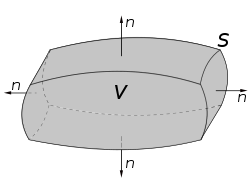
\includegraphics[scale=0.6]{div.png}
    \end{center}
\end{theorem}







\end{document}